\documentclass[12pt, a4paper, twoside]{article}

%% Preamble
\usepackage{umatfgspanish}
\usepackage[backend=biber]{biblatex}
\addbibresource{bibliografia.bib} 
\usepackage{subfiles}
\usepackage{blindtext}
\graphicspath{ {./images/} }



\begin{document}


%% Front Cover
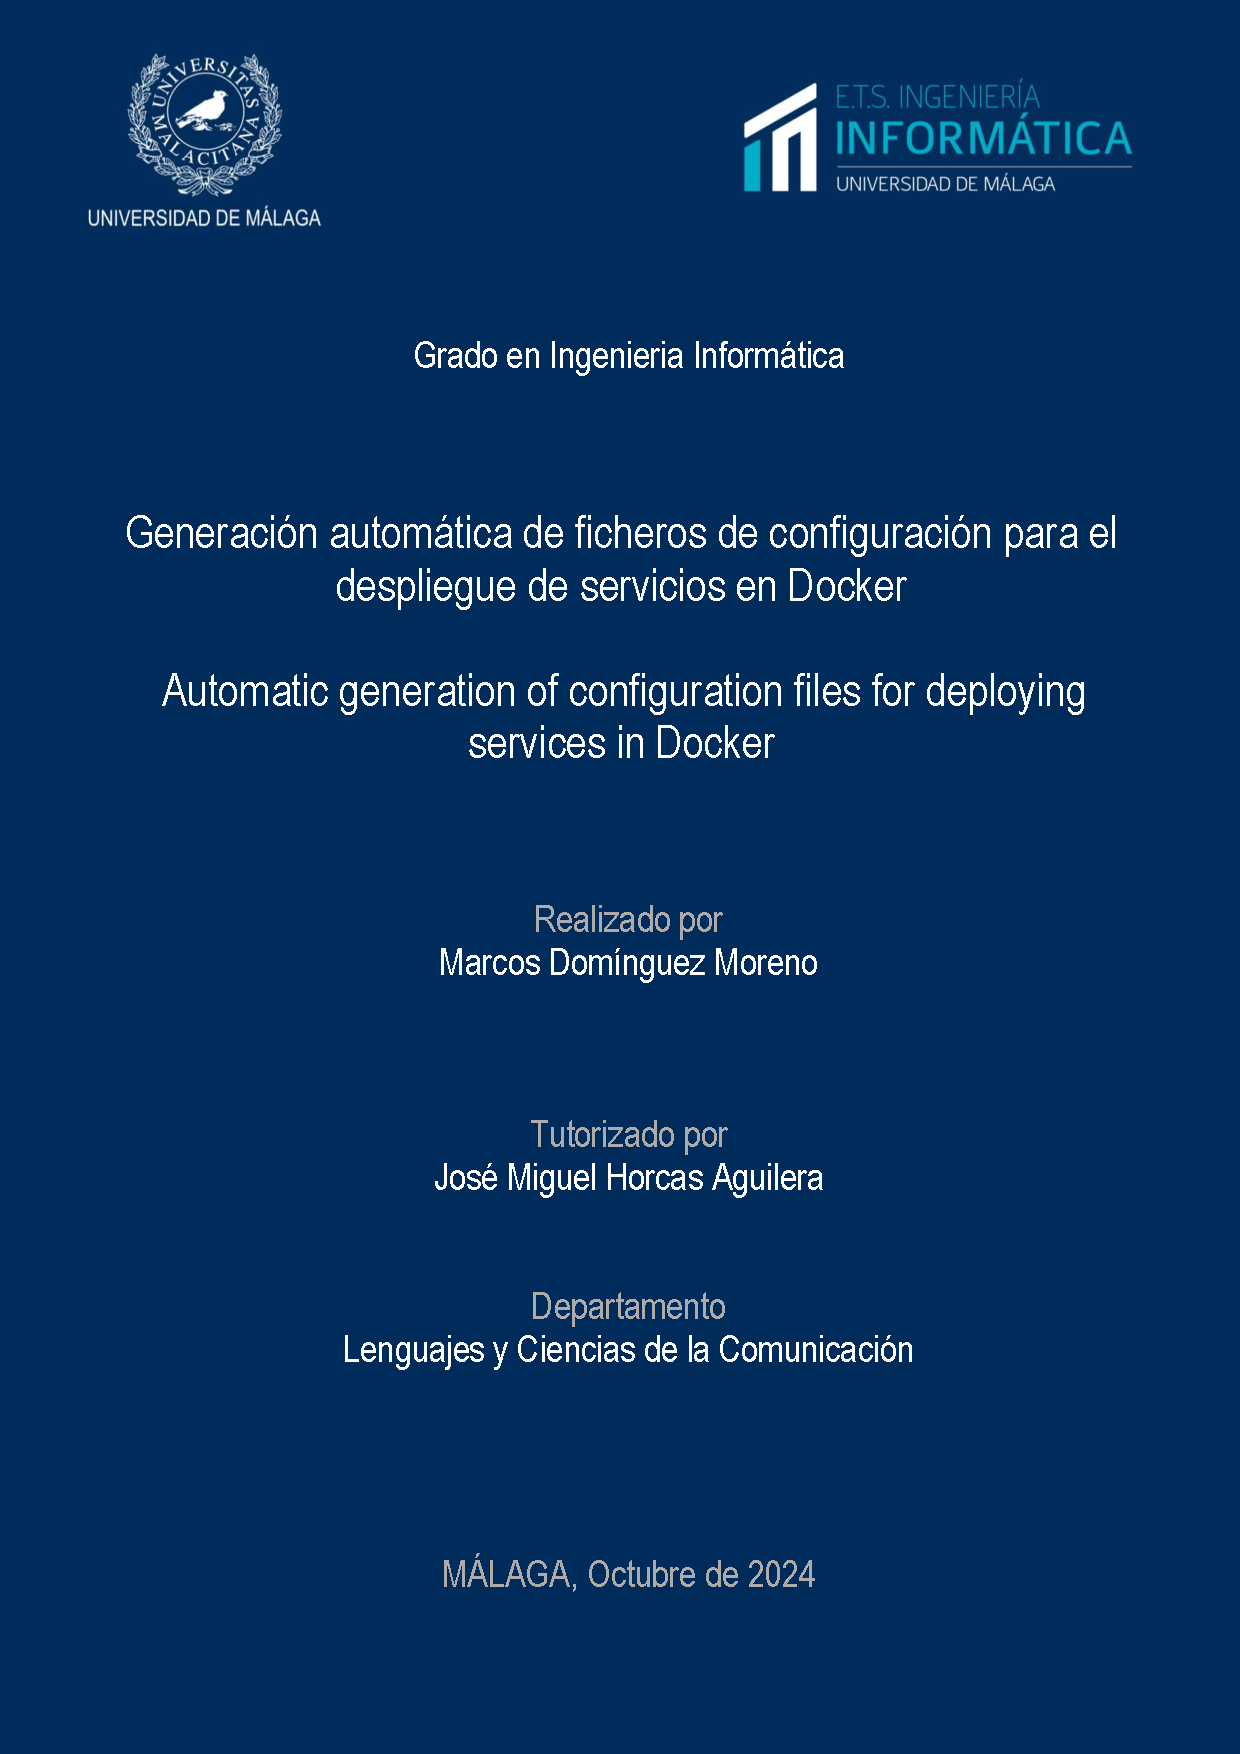
\includepdf[noautoscale=true, width=\paperwidth]{Portada-Titulo-Contraportada/cover.pdf}
\newpage

%% Title Page
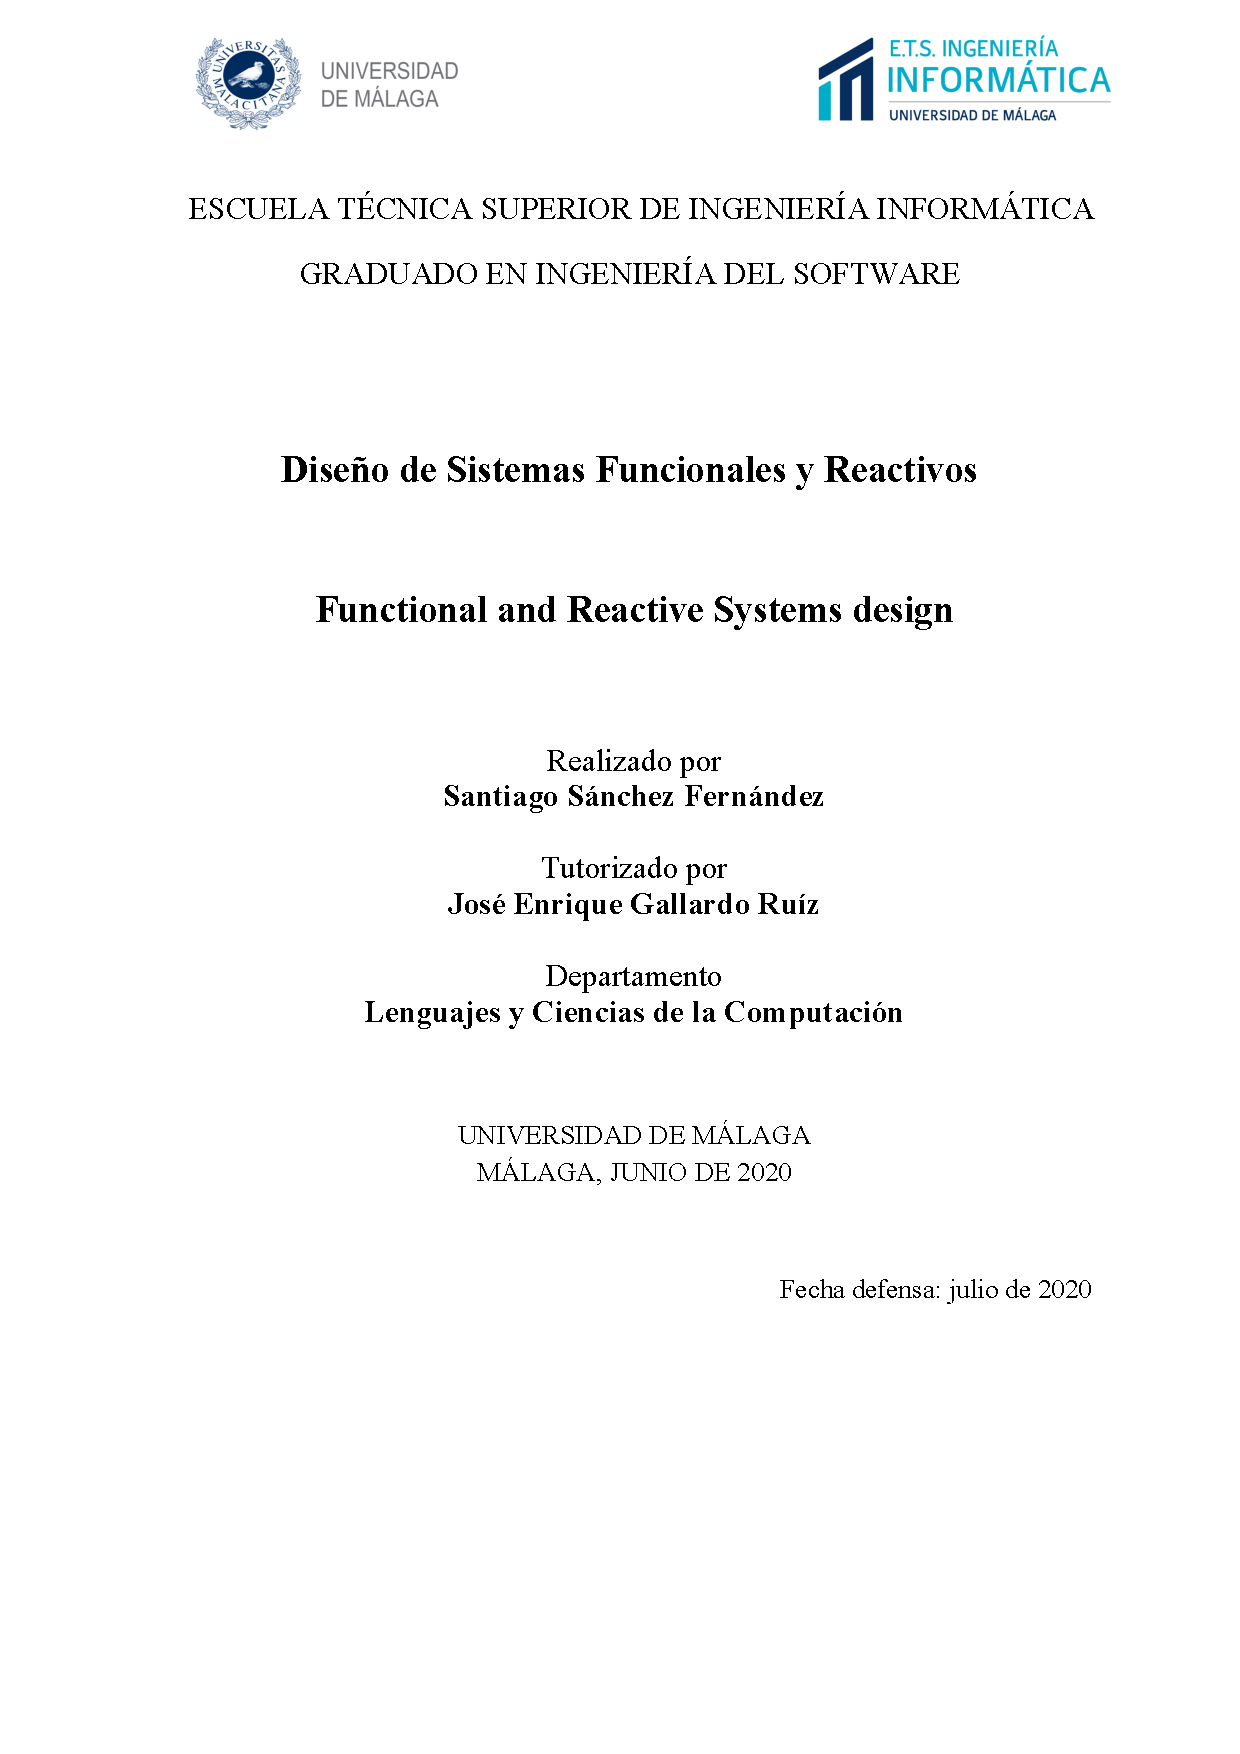
\includepdf[noautoscale=true, width=\paperwidth]{Portada-Titulo-Contraportada/title.pdf}

%% Abstract
\subfile{sections/abstract}
\newpage

%% Resumen
\subfile{sections/resumen}
\newpage

% Table of Contents
\tableofcontents
\newpage








%% Introduction
\section{Introduction}

\subsection{Motivación}
Las herramientas de automatización de tareas son fundamentales en el desarrollo de software, ya que permiten mejorar la eficiencia, la calidad y la consistencia en la producción de código.
Al relegar tareas repetitivas y propensas a errores a herramientas automatizadas, los desarrolladores pueden centrarse en tareas más creativas y de mayor valor añadido.
Parte del ciclo de vida en un desarrollo de software implica la configuración y el despliegue de servicios en entornos de producción y desarrollo.
La configuracion y despliegue requiere de la creación de archivos de configuración específicos, como los archivos Dockerfile y .dockerignore, que definen cómo se construye y se ejecuta una aplicación en un contenedor de Docker.
En el contexto de la tecnología de contenedores, Docker se ha convertido en una de las plataformas más populares para la creación, el despliegue y la gestión de aplicaciones en entornos contenerizados. 
Sin embargo, la configuración de servicios en Docker puede ser una tarea compleja y propensa a errores, especialmente cuando se manejan múltiples servicios y configuraciones personalizadas.
La motivación para realizar este proyecto surge de la necesidad de simplificar y automatizar el proceso de generación de archivos de configuración para el despliegue de servicios en Docker. 
En la actualidad, la creación manual de estos archivos dockerfile puede ser una tarea tediosa y propensa a errores al no conocer el usuario de toda la informacion necesaria para la correcta configuracion de los servicios, 
Al desarrollar una herramienta que automatice este proceso, 
se busca mejorar la eficiencia y la precisión en la configuración de entornos de contenedores, facilitando así el trabajo de desarrollo y administracion. 

\subsection{Objetivos}
El objetivo principal de este proyecto es desarrollar una herramienta que permita la generación automática de archivos de configuración para el despliegue de servicios en Docker.

\subsection{Resultados Esperados}
Dada la gran cantidad de opciones de configuración disponibles en para la generacion de ficheros de configuracion como puedes ser dockerfile..., el desarrollo de esta herramienta presenta varios desafíos técnicos y conceptuales.
El primero de ellos es la magnitud de las opciones de configuración disponibles, que pueden variar en función de las necesidades y los requisitos de cada servicio.
dar una covertura a todos los escenarios posibles es una tarea inabarcable, por lo que se ha optado por centrarse en los casos de uso más comunes y en las configuraciones más utilizadas en la práctica.
Sin embargo se espera que la herramienta sea lo suficientemente flexible y extensible como para permitir la incorporación de nuevas plantillas y configuraciones en el futuro.


\subsection{Estructura del documento}
Por definir










%% Estado del Arte 
\section{Estado del Arte}
Para la realización de este proyecto se ha realizado un estudio del estado del arte en el ámbito de la generación de archivos de configuración para el despliegue de servicios en Docker.
En este apartado se presentan las principales herramientas y tecnologías disponibles en la actualidad, así como las tendencias y los enfoques más comunes en la configuración de servicios en entornos de contenedores.
\subsection{Contenedores}
Los contenedores son paquetes ligeros que incluyen el código de las aplicaciones junto con sus dependencias, como versiones concretas de entornos de ejecución de ciertos lenguajes de programación y bibliotecas indispensables para ejecutar los servicios de software.
\subsection{Imagenes}
Las imágenes de contenedores son plantillas de solo lectura que contienen el código de la aplicación, las bibliotecas, las dependencias y otros archivos necesarios para ejecutar un contenedor.
\subsection{Docker}
Docker es un proyecto de código abierto que automatiza el despliegue de aplicaciones dentro de contenedores de software, proporcionando una capa adicional de abstracción y automatización de virtualización de aplicaciones en múltiples sistemas operativos
Docker es una plataforma de código abierto que permite a los desarrolladores crear, desplegar y ejecutar aplicaciones en contenedores. 
\subsubsection{Dockerfile}
El archivo Dockerfile es un archivo de texto que contiene una serie de instrucciones que Docker utilizará para construir una imagen de contenedor.
Usualmente la construccion de un archivo de configuracion se realiza a partir de una imagen base, que puede ser una imagen oficial de Docker o una imagen personalizada creada por el usuario.
A dicha imagen se añaden las instrucciones necesarias para instalar las dependencias y configurar el entorno de ejecución de la aplicación, lo que viene a representar el contenido de un archivo Dockerfile.
\subsubsection{Buenas Prácticas}
Para la creacion de los ficheros dockerfile es recomendable seguir una serie de buenas practicas para garantizar la eficiencia y la seguridad en el despliegue de servicios en Docker.
Estas practicas se recojen en la documentacion oficial de Docker y en guias de buenas practicas de la comunidad de desarrolladores.
\subsection{Problematica}
La creacion de los ficheros dockerfile puede ser una tarea tediosa y propensa a errores, especialmente cuando se manejan múltiples servicios y configuraciones personalizadas.
\subsection{Alternativas Actualmente Disponibles}
En la actualidad existen varias alternativas para la generación de archivos de configuración para el despliegue de servicios en Docker (dockerfile)
\subsubsection{Docker init}
Docker init es el comando de Docker Desktop CITA que permite inicializar un proyecto con un archivo de configuración básico.
su funcionamiento consta de elegir una plantilla de proyecto y seleccionar las opciones de configuración deseadas.
Las opciones de configuracion se limitan a elegir el lenguaje de programacion y que comando se ejecutara al iniciar el contenedor.
\subsubsection{Docker Extension for Visual Studio Code}
La extension de Docker para visual estudio code CITA permite entre sus funcionalidades la generacion de los ficheros dockerfile y dockerignore.
su comportamineto es similar al de Docker init, permitiendo elegir el lenguaje de desarrollo del proyecto y que comando se ejecutara al iniciar el contenedor.
\subsubsection{Inteligencia Artificial}
En la actualidad existen soluciones que se apoyan en la inteligacia Artificial 
para la generacion de archivos de configuracion, y para la creacion 
de los ficheros dockerfile y dockerignore. La calidad de estas soluciones es variable y depende de la calidad de los modelos de lenguaje natural empleados y de la calidad del promp de entrada.
como https://magickpen.com/templates/128/ CITA o alternativas con propositito más general como chatgpt CITA
\subsubsection{phpdocker}
Tambien estan disponibles alternativas más epecificas como https://phpdocker.io/ CITA que permiten la generacion de archivos de configuracion para servicios en php.
\subsubsection{Starter}
herramienta open source como estarter CITA https://www.startwithdocker.com/ capaces de reconocer el lenguaje de programacion del proyecto y generar un archivo de configuracion basico.


\subsection{Conclusiones}
En este estudio se han recogido algunas de las principales herramientas y tecnologías disponibles en la actualidad para la generación de archivos de configuración.
Todas las herraminetas proponen mediante plantillas la generacion de los ficheros dockerfile y dockerignore, estas plantillas son limitadas y no permiten la personalizacion de las opciones de configuracion.
No obstante suponen un punto de partida para el desarrollo de aplicaiones 

\subsection{Que se aporta en este contexto:}
Las opciones actualemtne disponibles para la generacion de archivos de configuracion para el despliegue de servicios en Docker son limitadas y no permiten la personalizacion de las opciones de configuracion.
Se deja de lado la variabilidad y las posibles opciones que existen a la hora de construir las imagenes, el proyecto proporcinara una nueva forma de construir plantillas dotando capacidad al usuario de una personalizacion
más profunda y detallada de las opciones de configuracion de los servicios en Docker.
















%% Tecnologías Empleadas
\section{Tecnologías Empleadas}
Este apartado describe las tecnologías y herramientas empleadas más relevantes para el desarrollo del proyecto, así como su función y su relación con el objetivo del proyecto.
Para el interes del lector 

\subsection{Universal Variability Language UVL}
CITA 
La Universal Variability Language (UVL) es un lenguaje de modelado diseñado específicamente para representar y manejar la variabilidad en sistemas software. 
La variabilidad en software se refiere a las partes de un sistema que pueden personalizarse, configurarse o cambiarse para adaptarse a diferentes necesidades o contextos. 
UVL se usa comúnmente en el contexto de ingeniería de líneas de productos de software (Software Product Line Engineering o SPLE), donde se trabaja con una familia de productos que comparten un núcleo común, pero pueden tener variaciones.

\subsubsection{Feature Models}
CITA 
El principal artefacto para modelar la variabilidad en SPL son los modelos de variabilidad. Existen muchos modelos 
de variabilidad pero los más extendidos y usados en la práctica son los modelos de características (feature models). 
Un feature model (FM) es un modelo para representar la variabilidad de una SPL en base a características comunes y 
variables (véase Figura 1), especificando qué características se pueden seleccionar en una configuración para generar 
un producto válido de la SPL
\subsection{Docker}
Con el objetivo de desarrollar una aplicaicon con animo de ejecutarse en contendores se ha optado por la tecnologia de Docker.
\subsubsection{Docker Desktop}
Para el manejo de los contenedores en el entorno de desarrollo se ha optado por la utilizacion de Docker Desktop.

\subsection{Node}
CITA
para el desarrollo de la aplicacion web se ha optado por la utilizacion de Node como entorno de ejecucion de JavaScript.
\subsection{Angular}
CITA
Para el desarrollo de la aplicacion web se ha optado por la utilizacion de Angular como framework de desarrollo de aplicaciones web.
\subsubsection{Angular Material}
CITA
CITA Para el diseño de la interfaz grafica de la aplicacion web se ha optado por la utilizacion de Angular Material como libreria de componentes.
\subsubsection{Monaco Editor}
CITA Para la edicion de los archivos de configuracion se ha optado por la utilizacion de Monaco Editor como editor de codigo.
\subsubsection{ngx-json-viewer}
CITA
CITA Para la visualizacion de los archivos de configuracion se ha optado por la utilizacion de ngx-json-viewer como visor de archivos json.

\subsection{Nginx}
CITA
Para el despliegue de la aplicacion web se ha optado por la utilizacion de Nginx como servidor web.
\subsubsection{Reverse Proxy}
CITA
Para el despliegue de la aplicacion y requerimientos adicionales se ha empleado Nginx como un proxy inverso.
\subsubsection{Web Server}
CITA
Para el despliegue de la aplicacion web se ha optado por la utilizacion de Nginx como servidor web.

\subsection{Python}
Para el desarrollo de los servicios de backend se ha optado por la utilizacion de Python como lenguaje de programacion.
\subsubsection{Flask}
Para el desarrollo de los servicios de backend se ha optado por la utilizacion de Flask como framework de desarrollo de aplicaciones web.
\subsubsection{guinicorn}
Para el despliegue de los servicios de backend se ha optado por la utilizacion de guinicorn como servidor web.
\subsubsection{Pypi}
Para la gestion de dependencias se ha optado por la utilizacion de Pypi como repositorio de paquetes de Python.

\subsection{Jinja}
\subsubsection{Jinja2}


\subsection{Git}
Para el control de versiones se ha optado por la utilizacion de Git como sistema de control de versiones.
\subsection{GitHub}
Para el almacenamiento de codigo se ha optado por la utilizacion de GitHub como plataforma de desarrollo colaborativo.
\subsubsection{GitHub Public Api}
Para la gestion de los repositorios de GitHub se ha optado por la utilizacion de la API publica de GitHub.
\blindtext

\subsection{Visual Studio Code}
Para el desarrollo de la aplicacion se ha optado por la utilizacion de Visual Studio Code como entorno de desarrollo integrado.
\subsubsection{UVLS extension}
Para la edicion de los archivos de configuracion se ha optado por la utilizacion de la extension de UVLS para Visual Studio Code.
ademas de las siguientes extensiones:
EXTENSIONES VISUAL ESTUDIO
	-UVLS https://github.com/Universal-Variability-Language/uvl-lsp
	-Docker
	-Flama https://marketplace.visualstudio.com/items?itemName=diversolab.flamapy
	-Graphiz Inetractive Preview https://marketplace.visualstudio.com/items?itemName=tintinweb.graphviz-interactive-preview
	-Latex Worshop
	-Pylance
	-Python
	-Python Debugger
	-Better Jinja






%% Metodología
\section{Metodologia del trabajo. (Fases) Implementación:}
\subsection{Introduction}
El enfoque se ha dado en desarrollo de este trabajo ha consistido en combinar un trabajo previo de analisis e investigacion con un desarrollo iterativo y agil.
La investigacion y analisis previo teniea el objetivo de conocer en profundidad las tecnologias y herramientas empleadas
para porstesiromete estudicar una posible aplicacion de estas ideas y conceptos en el desarrollo de las plantillas.
una vez resuelta esta primera parte se ha procedido a una toma de requisitos y a la planificacion del desarrollo de la aplicacion.
para la implementacion de la aplicacion se ha optado por la utilizacion de una metodologia de desarrollo agil que permita la adaptacion a los cambios y la evolucion del proyecto.
\subsection{Metodología del Desarrollo}
Al encontrarnos ante un trabajo individual toda la responsabilidad y capacidad del desarrollo recae sobre una persona. 
Para el desarrollo de código optaremos por una metodología Scrum simplificada. De forma iterativa se ejecutará un Sprint con 
unos objetivos de desarrollo y planificación muy limitados. Con el objetivo de dar cabida a la complejidad del proyecto, 
con animo de encajar nuevas ideas y revisiones que pudieran sucederse.
Tras cada Sprint se evaluará la progresión y dirección del proyecto con el tutor. 
\subsubsection{Justificación}

El desarrollo de las plantillas requiere un estudio con el fin de limitar las opciones de configuración y centrarse en los casos de uso más comunes y en las configuraciones más utilizadas en la práctica.
De entrada aportar una solucion tecnica optima a un problema es extremadamente improbable, por lo que se opta por una metodologia de desarrollo agil que permita la adaptacion a los cambios y la evolucion del proyecto.
\subsubsection{Procedimiento}
Tras cada Sprint se evaluará la progresión y dirección del proyecto con el tutor. 
\subsubsection{Limitaciones}
El desarrollo de un proyecto de estas características requiere de una planificación y una metodología de trabajo adecuada.
En este sentido, como se han identificado anteriormente una serie de limitaciones y restricciones que pueden afectar al desarrollo del proyecto.
para el caso el desarrollo de las plantillas tiene que verse limitado en cuanto a formato y contenido, ya que no se puede abarcar todas las posibles opciones de configuracion.
\subsubsection{Fases de Estudio}
\subsection{Estudio del Estado del Arte :}
En esta fase se realiza una revisión exhaustiva de la literatura y tecnologías existentes relacionadas con el tema del 
proyecto. El objetivo es comprender el panorama actual, identificar tendencias, mejores prácticas y tecnologías 
relevantes que puedan influir en el desarrollo del proyecto.
\subsection{Investigación opciones de configuración para Docker}
Esta fase implica investigar y evaluar las diferentes opciones de configuración disponibles en Docker para el desarrollo 
y despliegue de aplicaciones. Se exploran las características, herramientas y técnicas que pueden optimizar el uso de 
Docker en el proyecto [2].

\subsection{Desarrollo Modelos plantillas dockerfile y dockerignore …}
Esta fase implica la construcción el árbol de características y las restricciones textuales que orienten el espacio de 
configuraciones posibles del fichero Dockerfile 

\subsection{Fase desarollo Scrum}
\subsubsection{Requisitios de la aplicación }
Aquí se definen y documentan los requisitos funcionales y no funcionales de la aplicación. Se recopilan y analizan las 
necesidades de los posibles usuarios, los objetivos del proyecto y las restricciones técnicas para establecer una base 
sólida para el desarrollo.
\subsubsection{Desarrollo del la aplicación de uvengine }
En esta fase se desarrolla la aplicación de uvengine, que permite la generación automática de archivos de configuración
\subsubsection{Desarrollo de la web}
En esta fase se desarrolla la aplicación web que permite la interacción con el usuario y la visualización de los archivos de configuración generados.
\subsubsection{Desarrollo de los servicios de backend}
En esta fase se desarrollan los servicios de backend que permiten la comunicación entre la aplicación web y la aplicación de uvengine y los repositorios.
\subsubsection{Elaboración de la guía de uso}
En esta fase se elabora una guía de uso que explica cómo utilizar la aplicación y las funcionalidades disponibles.
Se elabora una guía detallada que describe cómo utilizar la aplicación, incluyendo instrucciones paso a paso, capturas 
de pantalla y ejemplos. 
\subsubsection{Elaboración de un manual de instalación}
En esta fase se elabora un manual de instalación que explica cómo instalar y configurar la aplicación en un entorno local.
\subsection{Elaboración de la memoria}
En esta fase se redacta la memoria o informe final del proyecto, que documenta todo el proceso de desarrollo, desde la 
planificación hasta la implementación y las lecciones aprendidas. La memoria incluirá el análisis de los resultados, 
conclusiones y recomendaciones para trabajos futuros. 



%% Arquitectura y Modelado del sistema
\section{Arquitectura y Modelado del sistema }
\subsection{Vision general de la arquitectura }
\subsection{Arquitectura de backend}
\subsection{Arquitectura de Frontend}



%% Extesivilidad de la aplicación
\section{Extensibilidad}
\subsection{Plantillas}
\subsubsection{Plantillas de Dockerfile}
\subsubsection{Plantillas de Dockerignore}


%% Despliegue de la aplicación
\section{Despliegue de la aplicación  }
\subsection{ Despliegue local }
\subsection{ Despliegue en la nube }


%% Resultados
\section{Resultados}
\subsection{Resultados Obtenidos}
\subsection{Viabilidad del proyecto}
Estamos limitados por la generacion de los fiechors de configuracion que nos proporciona la extension uvls
\subsection{Escalabilidad}

%% Conclusiones
\section{Conclusiones y líneas Futuras }
\subsection{Conclusion Personal,}
\subsection{Conclusiones del Desarrollo del proyecto}
\subsection{Contribuciones / Aplicaciones Prácticas}
\subsection{Desarrollo de nuevas plantillas }
\subsection{Continuación en el desarrollo de plantillas ya existentes}
\subsection{Mejorar la experiencia del usuario }








%%%% Sections
%%\section{One \\}
%%
%%\subsection{Motivation}
%%    \blindtext[2]
%%    
%%    \begin{figure}[ht]
%%      \centering
%%        
\includegraphics[width=0.5\textwidth]{xp}
%%      \caption{A diagram showing the iterations of extreme programming.}
%%    \end{figure}
%%    
%%    \blindtext[4]
%%
%%\section{Two \\}
%%    \blindmathpaper






% Imprimir la bibliografía
\printbibliography




%% Bibliografia
%%\begin{thebibliography}{9}
%%    \bibitem{latexcompanion} 
%%    Michel Goossens, Frank Mittelbach, and Alexander Samarin. 
%%    \textit{The \LaTeX\ Companion}. 
%%    Addison-Wesley, Reading, Massachusetts, 1993.
%%    
%%    \bibitem{einstein} 
%%    Albert Einstein. 
%%    \textit{Zur Elektrodynamik bewegter K{\"o}rper}. (German) 
%%    [\textit{On the electrodynamics of moving bodies}]. 
%%    Annalen der Physik, 322(10):891–921, 1905.
%%\end{thebibliography}




%%\end{document}















%% Apendices
\begin{umaappendices}
    \section{Manual de \\ Instalación}
	\subsection{Requisitos Previos}
	\subsection{Descargar el codigo fuente}
	\subsection{Configuracion del archivo Dockercomose}
	\subsubsection{Nginx reverse proxy}
	\subsubsection{frontend}
	\subsubsection{Repository Manager}
	\subsubsection{UV Engine resolver}
	\subsection{Construccion de los contenedores}
	\subsubsection{Github API}
	\subsection{Terminar el servicio}



    \section{Manual de Uso}
	\subsection{Inicio de la aplicacion}
	\subsection{Barra de Navegación}
	\subsubsection{About Page}
	\subsubsection{Help Page}
	\subsection{Seleccionar plantilla}
	\subsubsection{Seleccionar version de la platilla}
	\subsubsection{Cargar configuracion}
	\subsubsection{Descargar Fichero Generado}
	\subsubsection{Copiar Fichero Generado}


\end{umaappendices}


%% Back Cover

\includepdf[noautoscale=true, width=\paperwidth]{Portada-Titulo-Contraportada/backcover.pdf}
\end{document}



\end{document}